\documentclass[12pt,onecolumn,a4paper]{article} % document style report

%\usepackage {t1enc}                                  % use DC-Font with 8 bit
%\usepackage [latin1]{inputenc}                       % Codepage latin1


\usepackage[centertags]{amsmath}                      % include ams-packages
\usepackage{amsfonts}
\usepackage{amssymb}
\usepackage{amsthm}
\usepackage{longtable}
\usepackage{array}

\usepackage{overcite}                                 % superscript notation of references

\usepackage[pdftex]{graphicx}                  % Grafikpaket f�r Bilder laden
\usepackage{hyperref}                  % F�r Referenzerstellung
\usepackage{xspace}

\newcommand{\rb}[2]{\raisebox{#1ex}{#2}}
\newcommand{\meshal}{\textbf{\emph{M\rb{-.25}{e}\rb{-.35}{s}\rb{-.45}{h}}}%
\textsf{\rb{-0.3}{a}\rb{-.15}{l}y}%
\texttt{\rb{.2}{\reflectbox{Z}}\rb{.1}{e}r}\xspace}

\begin{document}

\begin{titlepage}

\DeclareGraphicsExtensions{.png,.pdf,.jpg}
{
\renewcommand{\baselinestretch}{1.5} \small\normalsize

\begin{center}
{\Huge \meshal}
\\ \vspace{2cm} {\Large Mesh Display and Analysis} 
\\ \vspace{1cm} Manual Version 0.4
\end{center}
}
\end{titlepage}

\tableofcontents
 
\titlepage
\section{Introduction}

\subsection{Purpose}
\meshal is a program for displaying unstructured grids, visualizing data on the
grid, as well as examining the structure of the grid.
It is an ever changing and ongoing project that has been in development since 2001.
Certain file schemes and names may bear a vague resemblance to those used by
\emph{Cool Graphics}, a program developed by Jamey Eason, but it's only because he
thought too loudly when he was beside me in the office.

\section{Input Files}

\meshal assumes that there is a model, defined by a set of vertices,
which is to be displayed.
Beyond that, everything is optional.
The vertices may be connected to form structures, specifically
cables, triangular elements, quadrilaterals, tetrahedra,hexahedra, prisms, 
or simple line segments.
Scalar data may be associated with every point on the grid and 
may be used to colour
any of the connected structures.
An auxiliary set of points may also be defined on which to display vector data,

Furthermore, the points may be divided into different 
regions which may have their
attributes independently manipulated.
Regions are delimited by tagged volume elements (see \S\ref{sec:voleles}),
or may be specified by
a range of vertices (see~\S\ref{sec:regfile}),
As well, all the structures formed by those vertices are part of the
region.
Vertices may belong to more than one region,
and there is at least one region in a grid.
If a region is not specified, all structures belong to the default region.
If there is a element direction file (\texttt{.lon} file), and no 
volume elements are tagged, elements with no direction will be region~0, 
and other elements will be region~1.

Surfaces may be formed from collections of two-dimensional elements.
Surfaces are defined by surface element files (see \S\ref{sec:surffile}).
Also, surfaces are defined if there are any 2D elements in an \texttt{elem}
file (see \S\ref{sec:elem}). 
In the latter case, 
the 2D elements are placed in different surfaces based on their region number.
Surfaces are independent of regions, and the relationship between the points
and model structures is described in the Fig.~\ref{fig:UML}.
\begin{figure}
\centerline{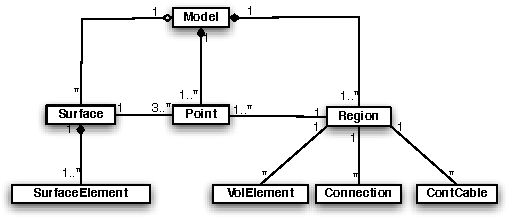
\includegraphics[width=13cm]{UML}}
\caption{Relationship between vertices (Points) and other structures.}
\label{fig:UML}
\end{figure}

All files (except IGB described below) are ASCII files.
They may be \emph{gzipped} 
in which case ``.gz'' should be appended to the extensions given below.
Note that files are scanned line by line 
and that extra information on each line is ignored by \meshal.

\subsection{Vertices}
\label{sec:pts}
The file defining vertices in the model is the only mandatory file.
It must have the extension ``.pts'' with the following format:
\begin{verbatim}
number_points
pt0.x pt0.y pt0.z
pt1.x pt1.y pt1.z
.
.
.
ptn.x ptn.y ptn.z
\end{verbatim}
The base name of this file, i.e., without the extension, is
used as the base name for cables, connections, triangles,
tetrahedra files, and shells files.

\subsection{Cables}
\label{sec:cabs}
Cables are vertices joined by a continuous line.
The points in a cable must be contiguous in the points file.
The file defining the cables
has the extension ``.cables'' with the following format:
\begin{verbatim}
number_cables
first_vertex_in_first_cable
first_vertex_in_second_cable
first_vertex_in_third_cable
.
.
.
first_vertex_in_last_cable
one_past_last_point_in_last_cable
\end{verbatim}
where the point indices are specified.
A cable will contain all points from the first specified in the cable until the
point before the first of the next cable.
\subsection{Connections}
Connections are line segments between vertices.
The file defining the connections
has the extension ``.cnnx'' with the following format:
\begin{verbatim}
number_connections
vertex#1 vertex#2
vertex#1 vertex#2
.
.
.
vertex#1 vertex#2
\end{verbatim}
where,again, the base-0 vertex indices are used and 
\subsection{Surface Elements}

\label{sec:surffile}
These files have the suffix ``.surf'' and
may define several surfaces in one file.
Any 2-dimensional element can be specified.
Labels are any sequence of characters not including white space.
The file has the following format:
\begin{verbatim}
number_elements_in_surface0 label_for_surface0 [label]
Tr vertex0 vertex1 vertex2 float
Qd vertex0 vertex1 vertex2 vertex3 float
.
.
.
Qd vertex0 vertex1 vertex2 vertex3 float
number_eleemnts_in_surface1 label_for_surface1 [label]
Tr vertex0 vertex1 vertex2 float
Tr vertex0 vertex1 vertex2 float
.
.
.
number_elements_in_surfaceN label_for_surfaceN [label]
Qd vertex0 vertex1 vertex2 vertex3 float
Tr vertex0 vertex1 vertex2 float
.
.
.
Tr vertex0 vertex1 vertex2 float
\end{verbatim}
where label is string without spaces which will be used to identify the surface in the list of surfaces.

\subsubsection{Triangles}
\label{sec:tris}
Triangle files are deprecated. 
They are defined in a file with the extension ``.tris'' or ``.tri''
which has the following format:
\begin{verbatim}
number_triangles_in_surface0 label_for_surface0
vertex0 vertex1 vertex2 float
vertex0 vertex1 vertex2 float
.
.
.
vertex0 vertex1 vertex2 float
number_triangles_in_surface1 label_for_surface1
vertex0 vertex1 vertex2 float
vertex0 vertex1 vertex2 float
.
.
.
number_triangles_in_surfaceN label_for_surfaceN
vertex0 vertex1 vertex2 float
vertex0 vertex1 vertex2 float
.
.
.
vertex0 vertex1 vertex2 float
\end{verbatim}
Thus, this file implicitly defines the number of shells in a model.
Currently, the fourth entry of the line is intended to be 
a material property indicator but it is unused.

\subsection{Volume Elements}
\label{sec:voleles}
There are two formats for defining volume elements, either the deprecated
tetrahedral file or the newer general element file. Details follow.

\subsubsection{Mixed element files}
\label{sec:elem}
Volume elements are specified by files with the ``.elem'' extension.
The element types and node orderings are given in Fig.~\ref{fg:voleledef}.
The file format is as follows:
\begin{verbatim}
number_elements
Hx n1 n2 n3 n4 n5 n6 n7 n8 [region]
Py n1 n2 n3 n4 n5 [region]
Pr n1 n2 n3 n4 n5 n6 [region]
Tt n1 n2 n3 n4 [region]
Tr n1 n2 n3 [region]
Qd n1 n2 n3 n4 [region]
.
.
.
\end{verbatim}
where \texttt{Hx, Py, Pr, Tt,Tr,Qd}
stand for Hexahedron, Pyramid, Prism,
Tetrahedron, Triangle and Quadrilateral respectively.
Each line may be any of the element types.
\begin{figure}
\centerline{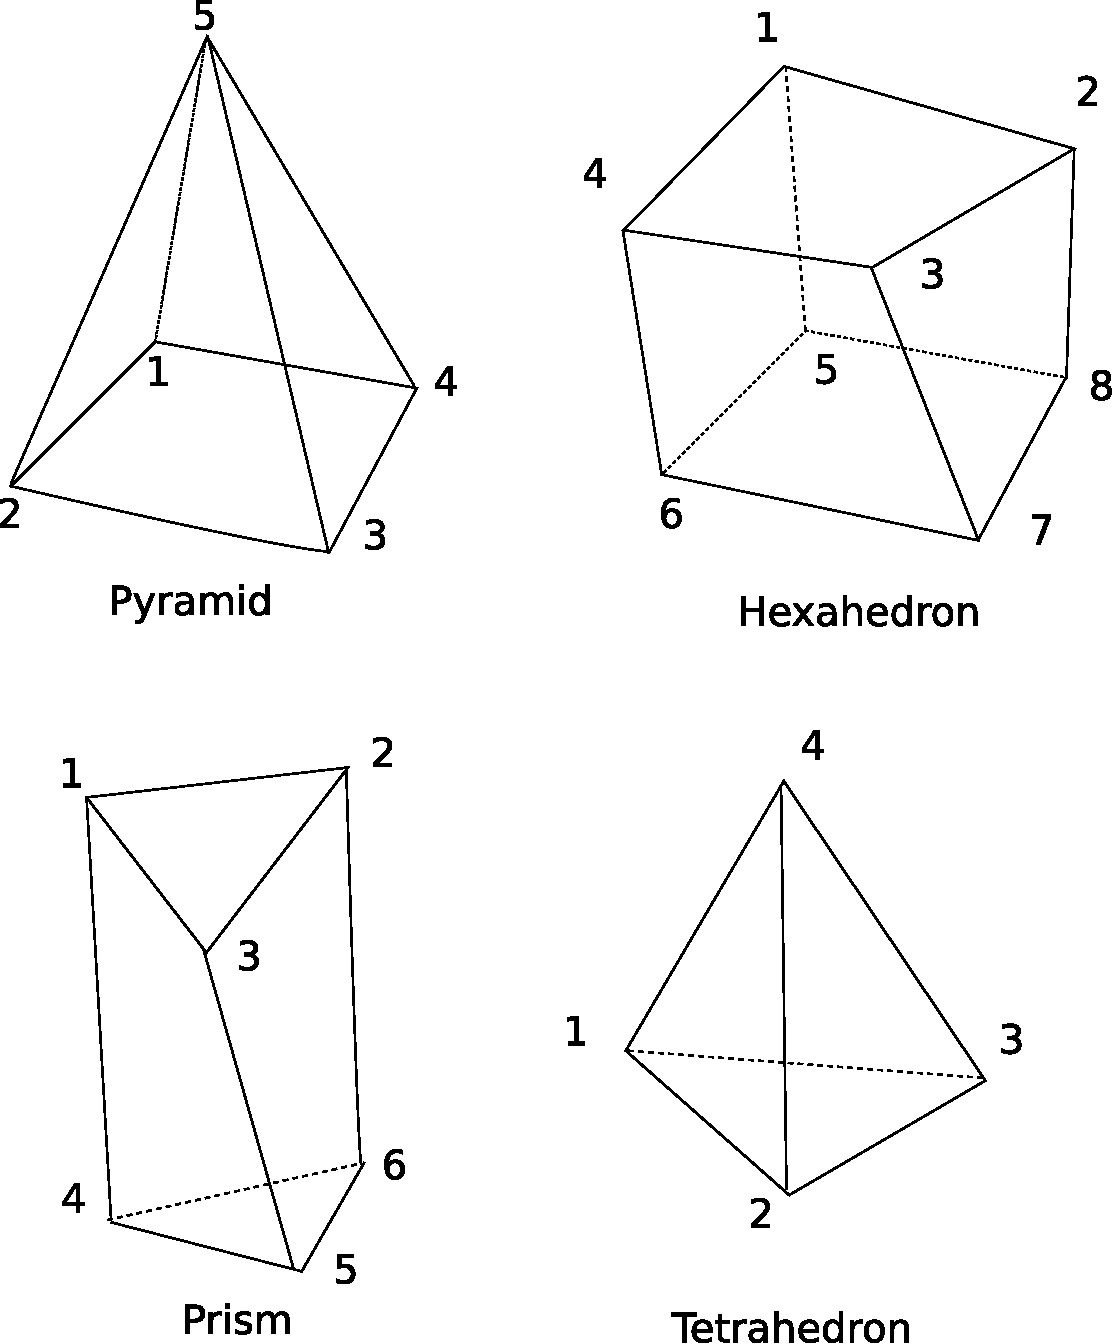
\includegraphics[width=10cm]{volelemdef}}
\caption{Volume elements\label{fg:voleledef}}
\end{figure}

\subsubsection{Tetrahedra}
\label{sec:tets}
Tetrahedra are defined in a file with a ``.tetras'' extension and the following
format:
\begin{verbatim}
number_tetrahedra
vertex0 vertex1 vertex2 vertex3 [region]
vertex0 vertex1 vertex2 vertex3 [region]
.
.
.
vertex0 vertex1 vertex2 vertex3 [region]
\end{verbatim}
The fifth entry of the line is a integer specifying a region. All nodes
of the tetrahedron belong to the region so nodes may belong to several
regions. If no region is specified, nodes are assigned to region 0.

\subsection{Regions}
\label{sec:regfile}
Regions may be explicitly specified in a separate file with the intention 
``.region''
with the following format:
\begin{verbatim}
number_regions
first_vertex_in_region0 last_vertex_in_region0
first_vertex_in_region1 last_vertex_in_region1
.
.
.
first_vertex_in_regionN last_vertex_in_regionN
\end{verbatim}

\subsection{Vertex Scalar Data}
Scalar data can be associated with each vertex.
It can be time dependent or a time independent.

\subsubsection{Time Independent}
A data file typically has the extension ``.dat'' or ``.out'' but these extensions
are suggested and not required.
The file simply contains lines with one entry per line, the data value for the
vertex.
\subsubsection{Time Dependent}
Files with time dependent data are typically suffixed with ``.tdat'' but this
extension is
not mandatory.
The file format follows that of the Static case, but is repeated for every time
instance.
Thus if there are N vertices and data is sampled at 10 points in time,
the file will comprise 10N lines with one value per line.

\subsubsection{IGB format}
\label{sec:IGB}
IGB is a format developed at the University of Montreal and used in a 
visualization program called flounder, for regularly spaced data.

The file is composed of a 1024-byte long header followed by binary data.
For irregular grids, the individual dimensions are meaningless but xdim$\times$ ydim$\times$ zdim should be equal to the number of vertices.
The header is composed of strings of the following format, separated by
white space:
\centerline{ \texttt{KeyWord:value} }
Note that the header must be padded to 1024 bytes.
The first block of key words need to be specified. The rest are optional.

\begin{longtable}{|l|l|p{0.7\textwidth}|}\hline
	KeyWord & Type & Description \\  \hline \endhead
    \hline \endfoot
    x       & int    & number of samples in x \\
	y       & int    & number of samples in y \\
	z       & int    & number of samples in z \\
	t       & int    & number of samples in t \\
	systeme & string & \texttt{big\_endian} or \texttt{little\_endian} \\
	type    & string & binary data type: byte, char, short, long,
	                   float, double, int, uint, vec3f, vec4f,
					   vec3d, vec4d\\ \hline
	unites  & string & units of data \\
	facteur & float & scaling factor for data \\
	zero    & float & data zero: true value =
	                            IGB\_data*\texttt{facteur}+\texttt{zero} \\
    org\_x  & float & lower right x coordinate       \\
	org\_y  & float & lower right y coordinate       \\
	org\_z  & float & lower right z coordinate       \\
	org\_t  & float & time of first slice            \\
	inc\_x  & float & distance between x samples \\
	inc\_y  & float & distance between y samples \\
	inc\_z  & float & distance between z samples \\
	inc\_t  & float & time between samples \\
	dim\_x  & float & extent in x \\
	dim\_y  & float & extent in y \\
	dim\_z  & float & extent in z \\
	dim\_t  & float & duration \\
	unites\_x & string & units of measure for spatial x dimension \\
	unites\_y & string & units of measure for spatial y dimension \\
	unites\_z & string & units of measure for spatial z dimension \\
	unites\_t & string & units of measure for time \\
    comment   & string & arbitrary comment \\
	aut\_name & string & author's name     \\
    transparent & hex & value for no data  
\end{longtable}
Note that for unstructured grids, $x$, $y$ and $z$ are meaningless. However, their product $xyz$ must equal the
number of nodes in the model.

\subsection{Vector Data}
To display vector data, an auxiliary set of points must be 
defined by a file with the ``.vpts'' suffix.
It follows the same format as the vertex file.
A file with the same base name but having the extension ``.vec'' defines the 
vector and scalar data. It has the following format:
\begin{verbatim}
data.x data.y data.z [scalar_datum]
data.x data.y data.z [scalar_datum]
.
.
.
data.x data.y data.z [scalar_datum]
\end{verbatim}
The scalar datum, as indicated, is optional.

Vector data can also be input as an IGB file using the types
\texttt{vec3f, vec4f, vec3d, vec4d} where 3 or 4 refers to the number of
elements in each datum,
and \texttt{d} and \texttt{f} refer to float or double.
The first 3 elements define the value of the vector field,
and the optional 4th element is the
scalar component as above. This file has the suffix ``.vec.igb''.

\subsection{Auxiliary Grid}
An auxiliary grid may be defined, optionally on which may be displayed
data. The grid may contain any of the elements forming the main grid
(points,lines,surface elements,volume elements), and the
elements may change as a function of time.
If scalar data has already been read in, the number of time instances in
the auxiliary grid must either be one, or the same as the scalar data.

A vertex file is mandatory and has the extension ``.pts\_t''.
An element file is optional. If present, it has the same base name as the
vertex file but with the extension ``.elem\_t''.
Scalar data may also be optionally defined on the auxiliary grid. The file
has the same basename as the vertex file but with the extension
``.dat\_t''.
The file formats follow:\\
\newcolumntype{A}{>{\ttfamily}l}
\begin{longtable}{|AAA|A|A|}\hline
    \multicolumn{3}{|l|}{base.pts\_t}& base.elem\_t & base.dat\_t \\
    \hline
    \multicolumn{3}{|l|}{\#times}& \#times & \#times \\ 
    \multicolumn{3}{|l|}{\#points\_time0} & \#elements\_time0 & \#data\_time0 \\
pt(0,0).x & pt(0,0).y & pt(0,0).z & element(0,0) & data(0,0) \\
pt(1,0).x & pt(1,0).y & pt(1,0).z & element(1,0) & data(1,0) \\
. & . & . & . & . \\
. & . & . & . & . \\
. & . & . & . & . \\
. & . & . & element(M,0) & . \\
. & . & . & \#elements\_time1 & . \\
. & . & . & element(0,1) & . \\
. & . & . & element(1,1) & . \\
. & . & . & . & . \\
pt(N,0).x & pt(N,0).y & pt(N,0).z & . & data(N,0) \\
  \multicolumn{3}{|l|}{\#points\_time1} & . & \#data\_time1 \\
pt(0,1).x & pt(0,1).y & pt(0,1).z & . & data(0,1) \\
pt(1,1).x & pt(1,1).y & pt(1,1).z & . & data(1,1) \\
. & . & . & . & . \\
. & . & . & element(M,1) & . \\
. & . & . & \#elements\_time2 & . \\
. & . & . & element(0,2) & . \\
. & . & . & . & . \\ \hline
\end{longtable}

\subsection{Dynamic Points}
Points may also move in space as functions of time.
This is often associated with displacement during contraction, for
example.
The number of points must remain constant for all time instances,
as well as the elements defined by them.
Dynamic point files use the IGB format (see \S\ref{sec:IGB}) with data type
\texttt{vec3f}. The extension for the file in this case is ``.dynpt''.

\subsection{HDF5 Format}
All of the previous data types may now be packaged into one HDF5 file. Reading and
writing of the data is done through an API so the data format will not be
described. The HDF5 file should have the suffix ``.datH5'' and may contain multiple
datasets of differing types.

\subsection{CG meta format}
Cool Graphics (CG) is a visualization program written chiefly by Jamey Eason
and its file format was pretty much copied for this program.
This format is kept for historical reasons and its use is deprecated.
There must be a vertex file (as previously described) and there
may a file for tetrahedra. These files must share a common basename.
\emph{Note that a major difference between CG format and the previously described
formats is that \textbf{CG vertex numbering starts at one instead of
zero}.}
This will not affect the vertex file but means that if the same grid is
described by the two formats, the tetrahedral indices for the CG file will
all be one greater than for the regular format.
In addition, there is a metafile listing the surfaces and
there may be a sequence of data files. 
The file formats for the metafile and data files follow.
\subsubsection{CG metafile}
This file must have the suffix ``.cg\_in'' and adheres to
the following format:
\begin{verbatim}
number_surface_files
0
surface_file_1
surface_file_2
.
.
.
surface_file_n
\end{verbatim}
where \texttt{surface\_files}
are triangle files (see section~\ref{sec:tris}) for
format) with the ``.tri'' extension. 
The extension is \emph{not} 
given in the CG metafile, eg, if the actual file name is \texttt{endo.tri},
only \texttt{endo} is given.
\subsubsection{Data files}
Data is given in a set of ASCII files with the extensions ``.t\#'' where
\texttt{\#} is the time of the data, i.e., it is composed of digits.
For each file, the format is
\begin{verbatim}
t = #
a b c
a b c
.
.
.
a b c
\end{verbatim}
where the first line indicates the time (\# same as in file extension)
and each line contains three data.
Currently, the first 2 are ignored but must be present.

\subsection{Temporal Data Agreement}
When temporal data is present, i.e., multiple frames of data exist for any
grid, the number of instances must agree for all grids loaded.
Given that one grid has $T$ frames of data where $T\ge2$, any grid can only
have 0, 1, or $T$ frames of data.
If there is one frame of data, it is always displayed.
Thus, for example, if the scalar vertex data was loaded and contained 
1 frame of data, an
auxiliary grid with 100 frames could be read in, and subsequently a
vector data grid could only be read if it had 1 or 100 frames of data.

\section{Invocation}
The program is run by typing
\begin{verbatim}
meshalyzer [otps] [pts [vpts] [dat|tdat|igb] [mshz] [tri ...] [pts_t] [dynpt]]
\end{verbatim}
where the extensions of the required file types are given.
If no file is specified, a file input box will pop up.
Note that for the ``pts'' file, the dot of the extension can be left in to facilitate
using tab completion. 
For example, if the vertices file was called \emph{model.pts},
one could specify ``model.pts'', ``model.'', or ``model'' equally on the command line.
This only applies to the vertex file.

\subsection{Options}

\begin{description}
    \item[--help] Display the usage message
    \item[--iconifycontrols]  iconify the control window on startup
    \item[--groupID=GID] Be part of this semaphore group for \meshal linking. See \S\ref{sec:link}.
    \item[--noelem] Do not read in the element file. This will speed up reading in the model at the expense of
        not being able to put data on the cutting planes.
    \item[--thrdRdr] Force threaded data reading. Even if one has enough memory to read in all the data at
        once, it is probably just as fast to read it in on demand. Using this option will reduce start up time
        and stop \meshal from using all the RAM.
    \item[--PNGfile] Output file name for PNG files or output directory name for PNG sequences
    \item[--frame] first frame for PNG output (-1=do not set)
    \item[--numframe] number of frames to output to PNG images (default=1)
    \item[--size] width (and height) of PNG in pixels (default=512)
\end{description}

Note that only enough characters to uniquely identify the option need be used.
See the Offscreen Rendering section\ref{sec:offscreen} for a complete description of how to use PNG related options.

\subsection{Environment variables}
\meshal reads the following environment variables:
\begin{description}
\item[MESHALYZER\_MODEL\_DIR] This is a colon separated list of directories
which will be searched for models. If a model is not found as
specified, the model will be searched relative to these directories.
Also, when \meshal is invoked with no model file, the chooser will open in
the first directory specified in the variable.
\end{description}

\section{Graphical User Interface}

\begin{figure}[htbp]
\centerline{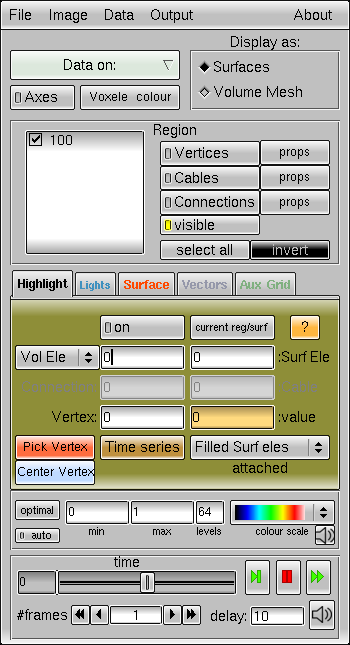
\includegraphics[width=8cm]{controls}}
\caption{The control widget.}
\end{figure}

\subsection{Volume Mesh}
To display the volume element mesh, click on the  \emph{Voxele Mesh} 
radio button in the
\emph{Display as:} box.
The colour of the volume elements can be changed with the \emph{Voxele colour}
button.
No other structure types will be displayed.

\subsection{Regions}
To not display the mesh as a set of volume elements,
click on the  \emph{Surfaces} 
radio button in the
\emph{Display as:} box.
This will display all structures except volume elements.

Display of each structure type can be toggled on and off on a
region-by-region basis or all-at-once.
The regions in which changes will take place are selected
by highlighting them in the list.
Any changes made to display structures will only occur to the regions selected.
The opacity value of a region
is changed by dragging in the opacity bar. It affects
all structures in a  region equally.
Sometimes rendering with opaque objects does not look quite
right because of drawing
order.
The order can be reversed by checking ``Reverse Draw order'' under the ``Image''
menu.

For each structure, there is a button toggling its display, 
and a button to select its display properties.
pressing the ``props'' button will open a widget to specify 
colour when it is not displaying data, to specify the output stride, size 
and if a 3D effect is to be used. 
Note that the 3D effect is graphics intensive and may be very slow for a 
large number of structures.

Different structures in different layers can be coloured differently.
Under ``Image/Randomly colour'', one can select which structure types gets randomly
coloured based on the region to which it belongs.
``Image/Background colour'' changes the colour of the background.

\subsection{Tab Widget}

\subsubsection{Highlighting}

Highlighting allows one to investigate the structure of the mesh.
One of each type of structure can be highlighted. 
A highlighted element is drawn in a special highlight colour.
The highlighted structure can be chosen by typing its number. Values can be changed
by using the up/down arrow keys and by dragging the mouse. See the FLTK manual for
a full explanation of the latter.
Pressing CTRL causes the arrow keys to increment by 10 while pressing
SHIFT causes them to increment by 100.
The mouse wheel can also be used with SHIFT and CTRL increasing the stride as well.
Hold both for a factor of 1000.
Volume elements can be selected to be drawn as a wireframe (\texttt{Vol Ele})
or a solid faced object (\texttt{Solid Vol Ele}).
Clicking on the ``current reg/surf'' button highlights the first
structure of each
type for the currently selected shell (0 if \emph{All} is chosen).

The highlighted vertex can also be selected with the mouse.
clicking on the ``Pick Vertex'' button will enter vertex picking mode
with the button turning red to indicate this.
A vertex can then be selected by clicking on it.
To properly pick a vertex, it is necessary to display vertices or 
outlined surfaces.
If you are having trouble selecting a vertex, display points, turn off all unnecessary
surfaces and regions, and click right on top of it.
In the event of nearby vertices, the one closest to the viewer's eye (minimum z
window coordinate) will be selected.
For each vertex, its associated scalar data value
is displayed in the gold widget.
You can choose to display the surface elements that the vertex is part of, or
the volume elements that it is part of.
The elements can be drawn as wireframe or with filled sides.
The inside surfaces of the sides (facing the node) 
will be coloured pink while the outside will be gold.

\subsubsection{Time Plot}
\label{sec:timeplot}
The time series at the highlighted vertex can be displayed by clicking the 
``plot time series'' button.
The current time is indicated by a vertical green line.
A trace can be saved by clicking on the ``Hold'' button.
Up to 8 traces can be saved this way.
To clear the held traces, click on mouse button 3 and select 
``clear static curves.''
The plotted traces can be saved in ASCII format by clicking
the ``Save'' button.
Normally, when a new point is clicked, the x and y range are recalculated
and the scale adjusted accordingly.
To prevent this behaviour, deselect the ``Autoscale'' button.
Within the time plot, a zooming rectangle can be selected with mouse button 1.
Clicking the middle mouse button will pop up the coordinates of the mouse.
Clicking on mouse button 3 will pop up a menu which includes ``reset view'' 
to rescale the graph and selections for setting the \emph{X} and \emph{Y}
range displayed.
\begin{figure}[htb]
\centerline{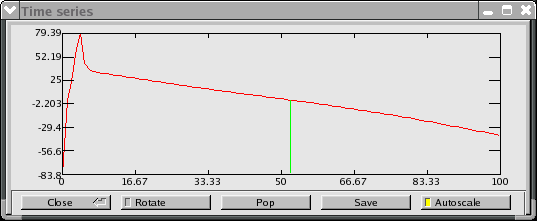
\includegraphics[width=10cm]{timeplot}}
\caption{Time series window.}
\end{figure}

\subsubsection{Information Window}
Clicking on the gold ``?'' button pops up a information window with details of the
selected structures.
For the highlighted node, all the structures of which it is a part are listed.
Clicking on any of those highlights them.
For each structure, the defining nodes are listed.
Clicking on any defining node causes that node to become the 
highlighted node.
For tetrahedra and triangles, the vertex scalar data values are displayed and for
tetrahedra, the solid angle of each node is also computed.

\subsubsection{Lighting}

Lighting is turned on with the \emph{illuminate} button and
only works well when a surface has been specified and either has
its vertices consistently ordered so that the normals 
point out when
calculated, or a normal file has also been read in.
The light is directional and its direction can be specified by the 3 sliders.
If \emph{fixed}, the light is constant and the object rotates.
If not \emph{fixed}, the light rotates with the object.
The direction of the light is graphically illustrated when the
``show direction'' button is on.
The intensity of the different lighting components can be adjusted with
the sliders.
With ``facet shading'' enabled, Gouraud shading is turned off and lines
are not antialiased. This may speed up rendering on slow platforms.

\subsubsection{Scalar Data}

\label{sec:scalardata}
Scalar data is read under the ``File'' menu in the top bar.
It can be static or time-dependent.
If time-dependent, animation can be played by clicking the green double arrow button
in the bottom panel.
The delay between frames in $\mu$s is selectable.
``\#frames'' selects how many frames to increment at a time.

If data is present, each vertex has associated scalar data which is linearly
mapped to a colour.
Clicking ``optimal'' maps the currently displayed minimum data value to 
level 0 and the currently displayed 
maximum data value to the maximum colour level.
The number of entries in the colour map is determined by the ``levels'' widget.
When ``auto cs'' is selected, the colour map is re-calibrated whenever the displayed
time changes.
It is equivalent to pressing ``optimal'' every time that time is changed.
The values corresponding to the minimum and maximum colour values are 
available for editing.

Different structures may be coloured according to the data.
The ``Data on:'' choice widget selects which structure types are coloured according
to the data values associated with the vertices defining the structures.

\subsubsection{Vector Data}

Vector data is specified on the command line or by selecting ``Read Vector Data''
under the ``File'' menu item.
Arrows are drawn at each vector grid point.
The size of all arrows can be scaled with the roller.
The relative length of the arrow can be based on the magnitude of the vector data,
by the optional scalar data value, or be fixed.
Colour can be based on vector magnitude, scalar data or be constant.
The constant value is selected by the ``colour'' button.
Magnitude and scalar data are mapped to a selectable colour map as with
vertex scalar data.
To display a subset of the data, a stride may be chosen.
Sometimes, especially with a regular grid is used, a constant stride will lead to aliasing effects. In this case,
checking the ``stochastic'' button will add a random perturbation to the stride so that the model is
irregularly sampled but on average, at the specified stride.

\subsubsection{Auxiliary Grid}

Auxiliary grids are specified on the command line or by selecting
``Read Aux Grid'' under the ``File'' menu.
The Dispaly button toggles drawing of the grid.
The colouring of the model components is controlled independently of the
main grid.
Widgets for selecting the colour scale and mapping of the scalar data to
colour are available. See \S\ref{sec:scalardata} for details.
Components are grouped into line, surface and volume elements.
Each group of grid components can be coloured with a fixed colour chosen
with the ``color'' button.
If scalar data is present, the components can be coloured according to the
associated data value, that is, ``datafied''.
The size of the components can also be controlled. For surface and volume
elements, the size refers to the line width when the components are drawn
as wireframe.
How the components are drawn can also be specified.

A node can be selected by entering its number in the provided widget on the
tab. 
The highlighting option must first be turned on.
Furthermore, if an auxiliary grid has the same number of vertices at all
instances of time, the time series of the vertex data can be displayed by
clicking on the ``Plot'' button.
See \S\ref{sec:timeplot} for a description of the widget.

\subsubsection{HDF5 data}

A file with the suffix ``.datH5'' can be read in. This file may contain many data
sets. Upon successfully opening the file, a dialog will open which displays the
data sets from the file which may be viewed on the current grid.

\subsubsection{Surfaces}

The fill colour of the elements composing surfaces can be selected as well
as the outline colour. Outlining and filling the elements can also be
controlled. In the surface tab, the surfaces to which the changes are
applied are chosen by the drop down menu.
Surfaces can also be randomly coloured by Image/Randomly Color/Surfaces.

\subsection{Image Menu}

\subsubsection{Reset Transform}
Restore the original default transformation.

\subsubsection{View}
Choose from standardized views. The first submenu indicates the axis which
is sticking out of the screen and the diagrams show the positive axes of
the other two dimensions.

\subsubsection{Randomly colour}

For each region, assign the same random colour to all of the element
types chosen.

\subsubsection{Background colour}

Select the background colour.

\subsubsection{Reverse draw order}

Draw the surfaces in the opposite order. This can be useful when surfaces
overlap and different perspectives are chosen.

\subsection{Data Menu}

\subsubsection{Data Opacity}
Data opacity is the ability to draw structures with an alpha value based on the
values of data associated with the structure.
For data below a minimum value, the data is draw with the ``minimum opacity''.
For data above a maximum value, it is drawn with the ``maximum opacity''.
In between the two data values, linear interpolation of the opacity values is used.
The opacity for each structure type is independent.
\begin{figure}[htb]
\centerline{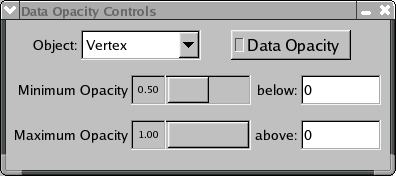
\includegraphics[width=8cm]{opacity_dialog}}
\caption{Data opacity dialogue.}
\end{figure}

A common use is the draw surfaces as translucent and then draw excited regions as
fully opaque.

\subsubsection{Clipping Planes}

By selecting ``Clipping'' from the ``Data'' menu item,
the clipping widget is popped open.
Six clipping planes are available.
They are defined by the normal to the clipping plane and the intercept of the
plane.
Only structures located on the side of the plane to which the normal points are drawn.
To flip the normal to point in the opposite direction, click on ``Flip''.
After adjusting the normal direction, click on ``Unitize'' so that
the normal has unit magnitude.
This ensures that when changing the intercept with the slider, one can move the
plane through the whole object.
For each clipping plane, several different modes are available:
\begin{description}
	\item[Off] The clipping plane is inactive and not visible
	\item[On]  The clipping plane is active but not visible
	\item[Whole Plane] The plane is active and can be seen
	\item[Intersection] The plane is on and can be seen only where it
		 intersects the object
    \item[Datafied] The plane is on, can be seen only where it
		 intersects the object, and if data is present and displayed,
		 will have data interpolated on to it. This surface will also be
		 affected by the ``Surface Opacity.''
 \end{description}
\begin{figure}[htb]
\centerline{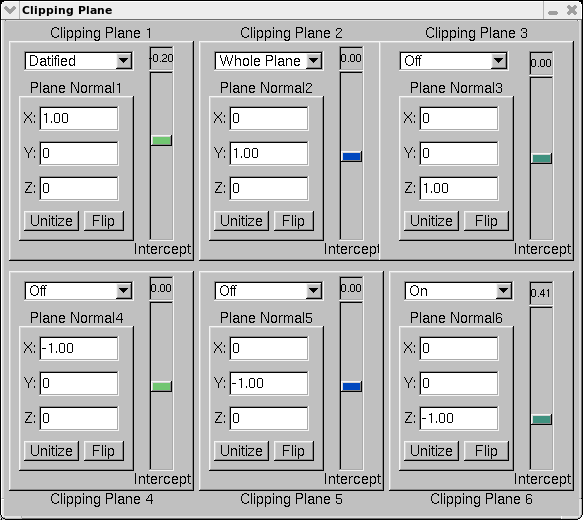
\includegraphics[width=12cm]{clip}}
\caption{Clipping plane dialogue.}
\end{figure}
At the bottom of the widget is a graphical interface for moving the clipping plane. 
The desired plane must first be selected.

\subsubsection{IsoSurfaces/IsoLines}

By selecting ``Isosurf'' from the ``Data'' menu item,
the isosurface/isolines widget is popped open.
This widget controls display of isovalue surfaces and lines.
Isosurfaces are only available if elements are defined. 
They are drawn with a specified colour and opacity.
Changes to the ``value'' are reflected when enter is pressed or the focus
changes.

For isolines, surfaces must be defined. An initial isovalue, ending
isovalue and the number of isovalue lines are specified.
If ``datified'' is selected, the lines are coloured according to 
the data colour scale, otherwise all lines are drawn with the same
specified ``colour''.
The thickness of the lines can also be controlled.

\subsection{Output Menu}

\subsubsection{Single Images}
Images can be saved in several formats under the ``Output'' menu.
Make sure that the window is unobstructed.
Formats that can be selected include PNG and
high quality vector EPS and PDF images.
With EPS and PDF, however, 
transparency is not supported due to a limitation of
the underlying third party software (GL2PS).
These images may be blown up to arbitrary size without pixelation effects.

\subsubsection{Animation Sequences}
For animation data, one can save a sequence of images in PNG format under the 
``Output'' menu.
For sequences, one selects a base name for the files and then 5 numbers for
the time frame number are appended, eg., image00012.png, image00013.png, etc.
These images are raster plots, based on the screen buffer, so larger 
windows will scale better.

\subsubsection{Recording Event Sequences}
It is possible to automatically write an image every time the contents of the window
change because of an event.
Thus, one can make a sequence of the model rotating or a sequence of the model as a
cutting plane is passed through it.
To begin recording, select ``Recording/start'' under the ``Output'' menu.
``Output'' will turn green to indicate that it is in recording mode.
As above, you will be prompted for a base file name which will have frame numbers
appended to it.
A blue ``Redraw'' label will also appear on the main menu bar.
Use this to force the output of the image, even if nothing has changed.
Manipulate the model any way you wish and when finished, select ``stop''.
A dialogue will pop up indicating how many frames were written.

\subsubsection{Visible nodes}

A list of the visible nodes and clipping planes can be generated by
selecting
``Output/Visible vertices''.
You will be prompted for a filename and a file with the following format
will be produced:
\begin{verbatim}
number_clip_planes_on
a1 b1 c1 d1
a2 b2 c2 d2
.
.
.
an bn cn dn
number_visible_vertices
visible_node1
visible_node2
.
.
.
visible_nodeN
\end{verbatim}
The coefficients (a,b,c,d) 
for the clipping plane are defined in the specified model coordinate system.

\subsection{Saving The Current View}

The current view can be saved by clicking on ``Save transform'' under the ``File'' menu.
You will be prompted for a file in which to save the current modelling transformation.
The current rotation, scaling and translation of the grid will be written to a file with
the extension \emph{.xfrm}.
Once saved, it can be restored later by choosing ``Read transform'' and selecting the file.

Standard views are available under the ``Image'' menu under ``View''.
The normal which points directly out of (+) or into (-) the screen is
first selected and then the positive direction of the other axes.

\subsection{Saving/Restoring the State}

The state is everything including the view transform. 
You can save the state under ``Save state'' in the ``File'' menu.
You will be prompted for a file which will have the extension \emph{.mshz}.
This file is text and can be edited by hand afterwards. 
You may delete any entries which you do not wish restored.
Upon invoking  \meshal from the command line, your home directory will be
searched for a default state file called \texttt{.default.mshz} 
which will be read in automatically.
A state file can also be specified on the command line and will supercede
any default settings.

\section{Grid window}

The grid is displayed in a window which has a virtual trackball.
Mouse button 1 (the left one for right-handed mice) rotates the grid.
Mouse button 2 translates the grid. This can also be achieved by pressing
\emph{SHIFT} while pressing mouse button 1.
Mouse button 3, or equivalently pressing \emph{CTRL} and mouse button 1,
changes the scale.

The axes showing the orientation of the window may be displayed by clicking on the
\emph{Axes} button.

The left and right arrow keys change the displayed time, one frame per press.

To recalibrate the colour scale to the optimal for the displayed data,
press ``o''.

Depressing the ``p'' key will enter vertex picking mode. It is a short cut for the
``Pick Vertex'' button.

To reread the current data file, press ``r''.

\section{Linking}

\label{sec:link}
Different \meshal instances can be linked together so that some operations are applied to all
instances.
To link instances of \meshal, click on ``File/Link'' which will open up a linking dialog 
listing all running instances of \meshal.
Linking is bidirectional so that linking a new process includes it in the group of currently
linked processes. As such, operations performed in any of the linked processes will be sent to
all processes.

Currently, linking supports the following operations:
\begin{description}
\item[Temporal changes] Increments or decrements in time will be transmitted to all instances. 
    This includes arrows and the animation button.
\item[Temporal syncing] Clicking on the ``sync'' button (beside the animation pause button)
      will set all instances to the same time. This is also achieved by pressing ``t'' in the
      model window.
\item[Viewport syncing] Clicking ``Image/Sync/Viewport Sync'' or pressing ``v'' in the model window 
     will transmit the current orientation, scale, and translation to all other instances.
 \item[Colour Scale] Clicking ``Image/Sync/Colour Scale Sync'', or pressing the sync button 
     beside the colour bar 
     will transmit the current colour map to all other instances.
\end{description}

\noindent
As a side effect of temporal linking, \meshal responds to the following UNIX signals:
\begin{longtable}{|l|l|}\hline
Signal & Action \\ \hline
SIGUSR1 & advance forward by the frame increment \\
SIGUSR2 & go backwards by the frame increment \\ \hline
\end{longtable}

If you wish to have different masters controlling different groups of slaves, you need
to specify a groupID on the command line for each group. The default is ``0''. 

\section{Offscreen Rendering}
\label{sec:offscreen}
Output PNG files may be written noninteractively. To do so, the \texttt{PNGfile} option must be specified. 
If one output frame is specified by setting \texttt{numframes} to 1, then \texttt{PNGfile}
is the output file name with ``.png'' appended
automatically if it is not specified. For more than 1 frame, \texttt{PNGfile} is a directory name, which will be created if
necessary, and the output files will have the names \texttt{frameXXXXX.png} where XXXXX is the frame number padded on the
left with zeros, eg., frame 8 would be ``frame00008.png''. Directory names will have ``.png'' stripped if detected on
the end. 
By default, the initial frame is not set, i.e., it will be that of a state file if one is read, or 0 if one is not
specified . 

The simplest way to use offscreen rendering is to set up meshalyzer in a suitable state and then save it. The model,
data and state files are specified as normal on the command line and the additional PNG related options added.
A simple example might be something like
\begin{verbatim}
meshalyzer --PNGfile=movie --numfr=10 --frame=5 myopurk.
        Vm.igb state.mshz
\end{verbatim}
which would produce 10 PNGs in the movie directory by putting the data in Vm.igb on the myopurk model and use the
setting in state.mshz. 

There are two version of \meshal for offscreen rendering. There is no differences in running the code but it is a
question of environment and speed.

\subsection{OSMesa}
OSmesa (http://www.mesa3d.org/osmesa.html) is an offscreen rendering library which performs all of its operations in
software. This has the advantage that it can be used even if a window server is not running. This library must be
available on the system. However, since it does not take advantage of the graphics hardware, rendering is considerably
slower. This executable must be explicitly compiled by
\begin{verbatim}
make mesalyzer
\end{verbatim}
with the resultant executable called \texttt{mesalyzer}. It cannot be used to display a window on the screen.

\subsection{GLUT rendering}
The GLUT library (http://www.opengl.org/resources/libraries/glut/) can be used to create an OpenGL context which then
allows offscreen rendering to use the graphics card. This is compiled into the default version of \meshal. It renders
very quickly but only if a windowing system is available. A small window with no content will be created that is a
byproduct of establishing a connection with the windowing system.

\end{document}
